% kapitel3.tex
\chapter{Randomized Load Aware Path Selection Algorithmus}
\label{chapter:algorithmus2}
\graphicspath{{../bilder/}}

Der Algorithmus Randomized Load-Aware Path Selection (RLAPS) ist ein heuristisches Routingverfahren, das entwickelt wurde, um Netzwerke gegen lokale Überlastung abzusichern und dabei dennoch kurze Pfade zu berücksichtigen. Anstelle deterministischer Shortest-Path-Strategien, die häufig zur Ausbildung von Hotspots führen, nutzt der Ansatz kontrollierte Randomisierung, um Diversität in der Pfadwahl zu erzeugen und dadurch den Datenverkehr gleichmäßiger im Netz zu verteilen. Ziel des Verfahrens ist es, eine einfach implementierbare und robuste Methode zur Lastverteilung bereitzustellen, die starke Auslastungsspitzen reduziert und die durchschnittliche Auslastung verbessert, ohne dabei anfällig für kleine Eingangsvariationen in Demands oder Topologie zu sein.

\section{Grundidee}

Die Grundidee besteht darin, für jede Demand zunächst eine Menge von k-kürzesten Pfaden zu berechnen. Aus dieser Menge werden anschließend drei Kandidaten zufällig ausgewählt und anhand einer lastbasierten Bewertungsfunktion beurteilt. Diese Funktion berücksichtigt die bereits auf den Links geplante Last sowie die jeweilige Kapazität und bestimmt so den Pfad, der die geringste zusätzliche Belastung erzeugt. Der beste der drei Kandidaten wird als endgültiger Pfad gewählt, die entsprechende Last auf den Links eingetragen und die lokalen Informationen über die Auslastung aktualisiert.

\section{Wie der Algorithmus funktioniert}

Kurzüberblick:

\begin{enumerate}
    \item Baue einen Graphen mit Kantenkapazitäten und optionalen Kantengewichtungen auf.
    \item Für jede Demand berechne eine Liste von k-shortest paths und wähle daraus 3 Kandidaten randomisiert (Oversampling).
    \item Bewerte jeden Kandidatenpfad anhand einer Lastfunktion, die die derzeit erwartete Linkauslastung berücksichtigt.
    \item Wähle den besten Pfad (minimaler Score). Trage die Last ein und aktualisiere die lokalen Lastinformationen.
\end{enumerate}

\section{Bewertungsfunktion}
Sei $P$ ein Pfad bestehend aus Kanten $(e_1,\dots,e_m)$ und $d$ die Demand-Größe. Mit $f_e$ der bisher auf $e$ geplanten Last und $c_e$ der Kapazität gilt die Pfadbewertungsfunktion

$$
\mathrm{score}(P,d) \,=\, \sum_{e\in P} \frac{f_e + d}{c_e}
$$

Diese Wahl zielt direkt darauf ab, die entstehende Auslastung auf den von $P$ genutzten Links zu minimieren.

\section{Pseudocode}
\begin{verbatim}
    for each demand (s,t,d):
    candidates = k_shortest_paths(G,s,t,K,oversample)
    sampled = random_sample(candidates, K)
    best = argmin_{p in sampled} score(p; d, flow\_map)
    assign best: update flow_map and G loads
    return waypoints, metrics (MLU, ALU, ...)
\end{verbatim}


\section{Experimente 1}

Im Rahmen der Experimente wurde der Algorithmus Randomized Load-Aware Path Selection (RLAPS) in die bestehende Testumgebung integriert. Die Implementierung selbst erwies sich vergleichsweise unkompliziert, da der Algorithmus im Kern nur auf der Berechnung von k-kürzesten Pfaden sowie einer einfachen Bewertungsfunktion basiert.
Das Ziel der Experimente bestand nicht allein darin, die maximale Linkauslastung (MLU) zu reduzieren, sondern auch die durchschnittliche Linkauslastung (ALU) zu verbessern. Durch die randomisierte Auswahl und die lastbewusste Pfadbewertung sollte der Algorithmus eine gleichmäßigere Lastverteilung im Netzwerk ermöglichen.


\section{Resultate 1}
Die Auswertung der Experimente erfolgte anhand der Metriken Average Normalized Link Utilization (ALU), Maximal Normalized Link Utilization (MLU) sowie der Ausführungszeit. Die Ergebnisse sind in den Abbildungen aus den Experimenten dargestellt.

In Bezug auf die durchschnittliche Linkauslastung (ALU) zeigt Abbildung 3.1 dass RLAPS im Vergleich im Mittelfeld liegt. Dennoch wird sichtbar, dass RLAPS einen Beitrag zur Reduzierung der durchschnittlichen Last im Netzwerk leistet und damit das angestrebte Ziel, neben der MLU auch die ALU zu verbessern, grundsätzlich erfüllt.

Betrachtet man die maximale Linkauslastung (MLU), so wird in Abbildung 3.2 deutlich, dass RLAPS in nahezu allen getesteten Topologien  eine Verringerung von Hotspots erreicht. Während einfache Verfahren wie Inverse Capacity oder Greedy Waypoints oft hohe Spitzenlasten verursachen, gelingt es RLAPS durch die randomisierte Pfadwahl und lastbasierte Bewertung, die maximale Auslastung einzelner Links abzufedern.

Ein weiterer Aspekt betrifft die Ausführungszeit, wie in Abbildung 3.3 dargestellt. Hier zeigt sich, dass RLAPS zwar deutlich langsamer arbeitet als einfache Verfahren wie Unit Weights, jedoch im Vergleich zu exakten den anderen Ansätzen erheblich schneller ist. Die Implementierung des Algorithmus ist zwar sehr simpel und benötigt lediglich lokale Lastinformationen, die Berechnung von k-kürzesten Pfaden und die wiederholte Bewertung mehrerer Kandidatenpfade führen jedoch zu einem deutlichen Mehraufwand. Besonders auffällig ist, dass die Rechenzeit mit wachsender Topologiegröße und komplexität exponentiell angestiegen ist, was die praktische Anwendbarkeit in sehr großen Netzwerken einschränken kann. Diese eingeschränkte Skalierbarkeit stellt damit eine der wesentlichen Limitationen von RLAPS dar.

\begin{center}
        \centering
        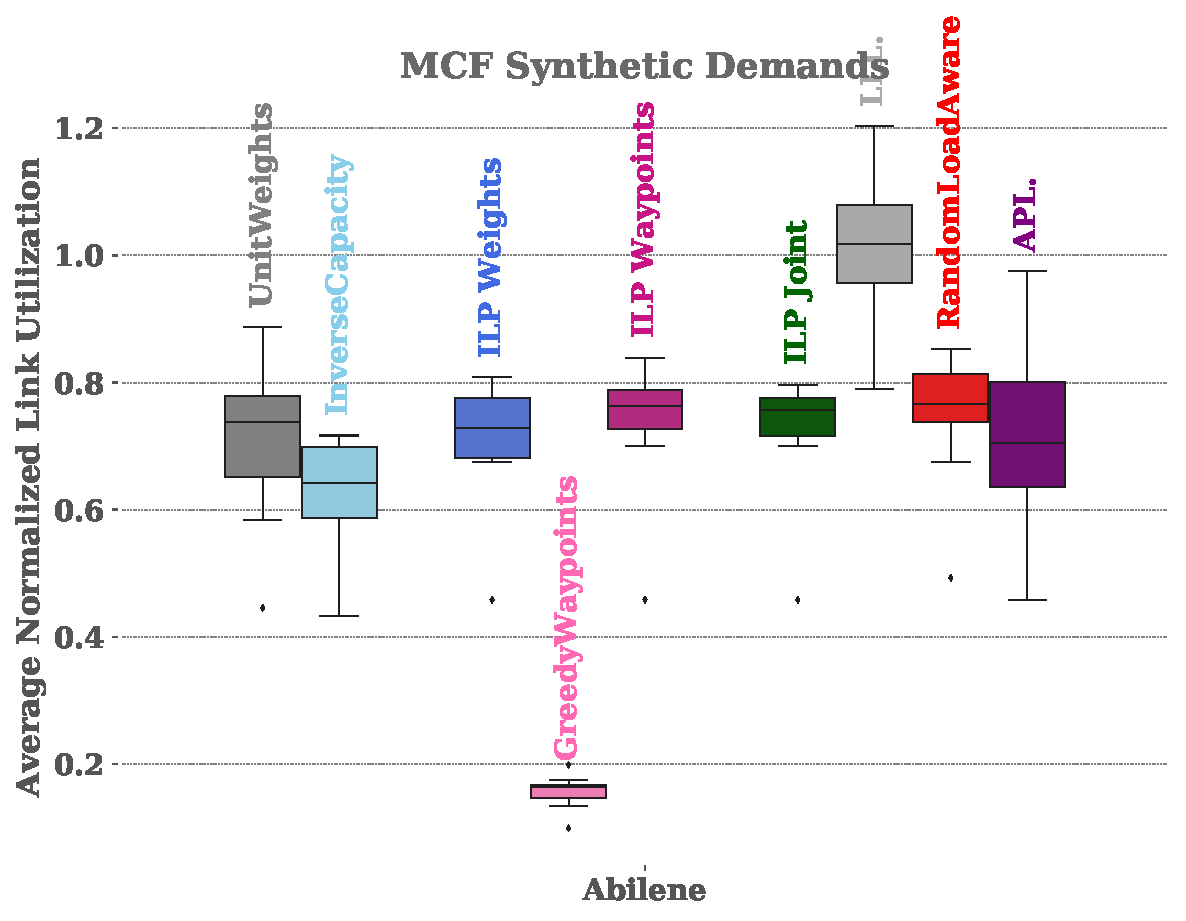
\includegraphics[width=\textwidth]{Report/bilder/RLAPS/all_algorithms_abilene_objective_alu.pdf}
        \small\textbf{Abb. 3.1:} Synthetische Demands ALU
        \label{fig:enter-label}
\end{center}

\begin{center}
        \centering
        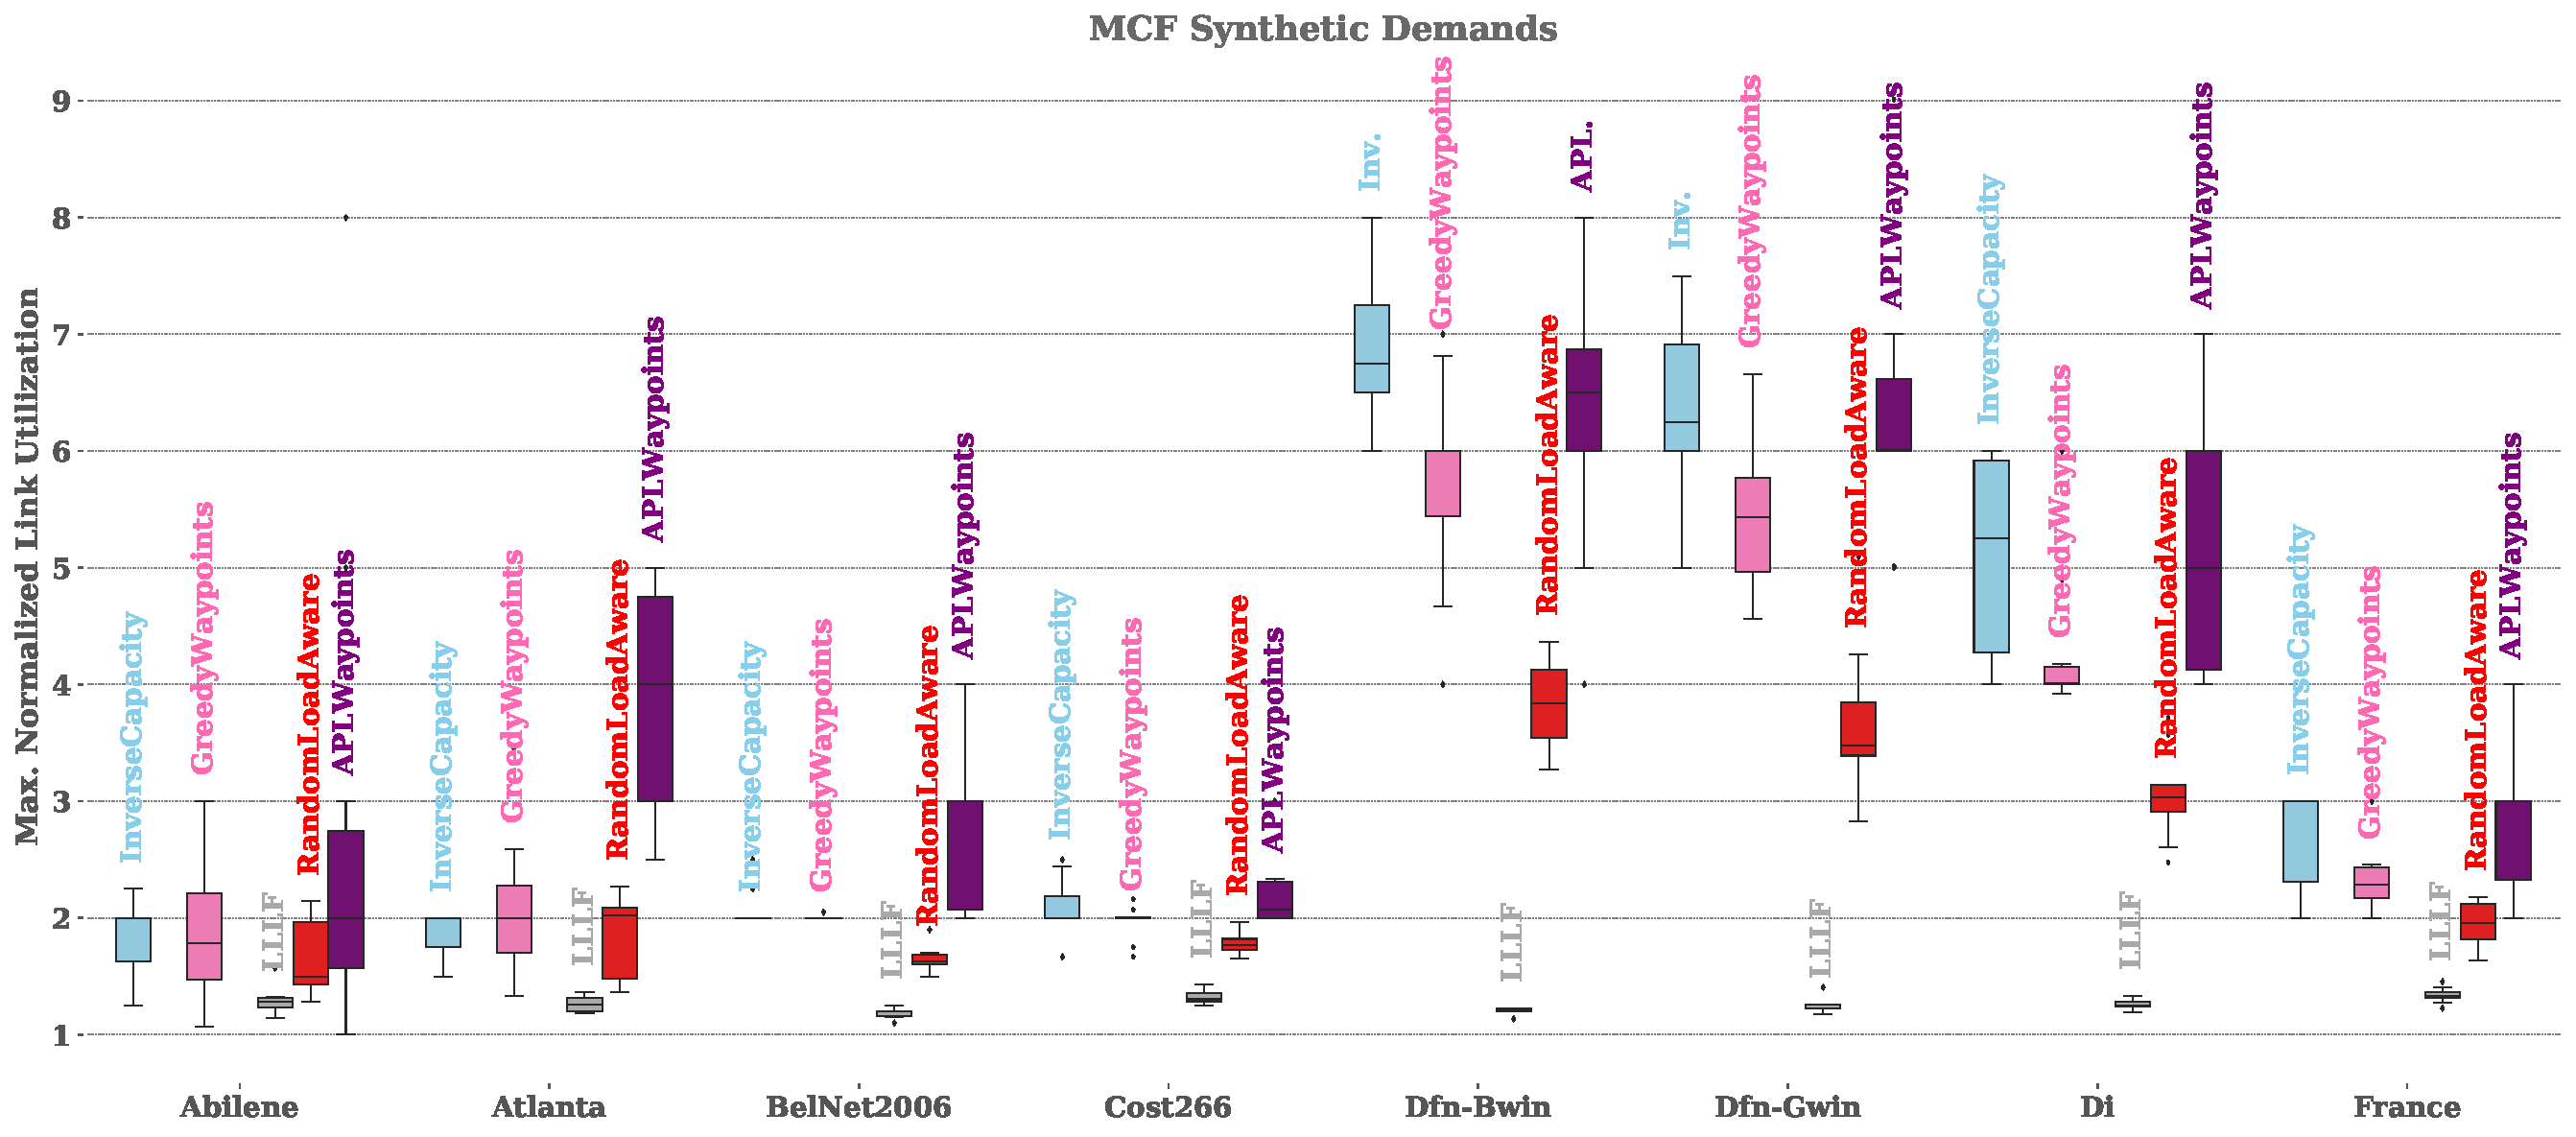
\includegraphics[width=\textwidth]{Report/bilder/RLAPS/all_topologies_objective_mlu_0.pdf}
        \small\textbf{Abb. 3.2:} Alle Algorithmen MLU
        \label{fig:enter-label}
\end{center}

\begin{center}
        \centering
        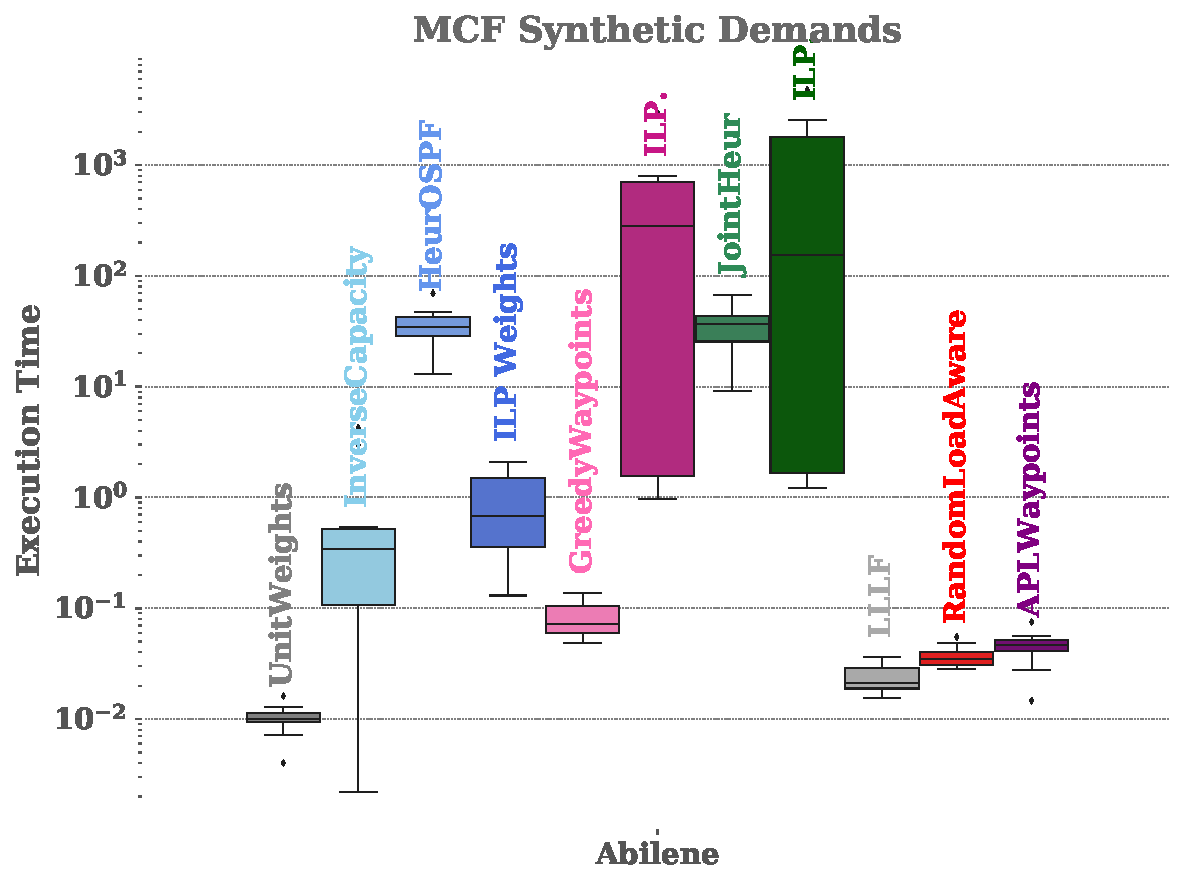
\includegraphics[width=\textwidth]{Report/bilder/RLAPS/all_algorithms_abilene_execution_time.pdf}
        \small\textbf{Abb. 3.2:} Alle Algorithmen Ausführungszeit
        \label{fig:enter-label}
\end{center}

\section{Experimente 2}

\begin{frame}{}
    
    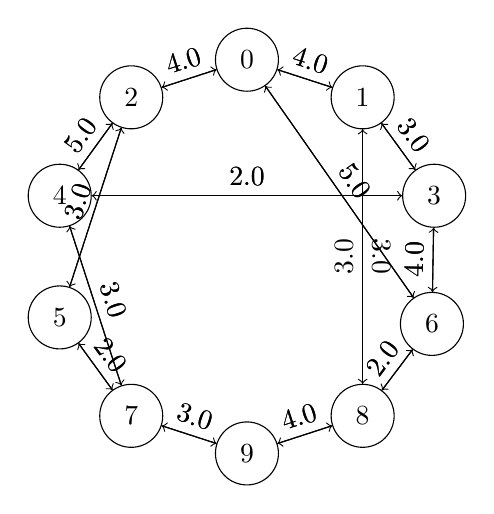
\begin{tikzpicture}[node distance=2cm, scale=1, transform shape]
        
        % Define custom style for nodes (only!)
        \tikzset{
          mynode/.style={circle, draw, minimum size=8mm}
        }
        
        % Define nodes in a circular layout
        \node[mynode] (0) at (90:2.5) {0};
        \node[mynode] (1) at (54:2.5) {1};
        \node[mynode] (2) at (126:2.5) {2};
        \node[mynode] (3) at (18:2.5) {3};
        \node[mynode] (4) at (162:2.5) {4};
        \node[mynode] (5) at (198:2.5) {5};
        \node[mynode] (6) at (340:2.5) {6};
        \node[mynode] (7) at (234:2.5) {7};
        \node[mynode] (8) at (306:2.5) {8};
        \node[mynode] (9) at (270:2.5) {9};
        
        % Draw directed edges with plain text labels for capacities
        \draw[->] (0) -- (1) node[midway, sloped, above] {4.0};
        \draw[->] (1) -- (0) node[midway, sloped, above] {4.0};
        \draw[->] (0) -- (2) node[midway, sloped, above] {4.0};
        \draw[->] (2) -- (0) node[midway, sloped, above] {4.0};
        \draw[->] (1) -- (3) node[midway, sloped, above] {3.0};
        \draw[->] (3) -- (1) node[midway, sloped, above] {3.0};
        \draw[->] (2) -- (4) node[midway, sloped, above] {5.0};
        \draw[->] (4) -- (2) node[midway, sloped, above] {5.0};
        \draw[->] (2) -- (5) node[midway, sloped, above] {3.0};
        \draw[->] (5) -- (2) node[midway, sloped, above] {3.0};
        \draw[->] (3) -- (4) node[midway, sloped, above] {2.0};
        \draw[->] (4) -- (3) node[midway, sloped, above] {2.0};
        \draw[->] (3) -- (6) node[midway, sloped, above] {4.0};
        \draw[->] (6) -- (3) node[midway, sloped, above] {4.0};
        \draw[->] (4) -- (7) node[midway, sloped, above] {3.0};
        \draw[->] (7) -- (4) node[midway, sloped, above] {3.0};
        \draw[->] (5) -- (7) node[midway, sloped, above] {2.0};
        \draw[->] (7) -- (5) node[midway, sloped, above] {2.0};
        \draw[->] (6) -- (0) node[midway, sloped, above] {5.0};
        \draw[->] (0) -- (6) node[midway, sloped, above] {5.0};
        \draw[->] (6) -- (8) node[midway, sloped, above] {2.0};
        \draw[->] (8) -- (6) node[midway, sloped, above] {2.0};
        \draw[->] (7) -- (9) node[midway, sloped, above] {3.0};
        \draw[->] (9) -- (7) node[midway, sloped, above] {3.0};
        \draw[->] (8) -- (1) node[midway, sloped, above] {3.0};
        \draw[->] (1) -- (8) node[midway, sloped, above] {3.0};
        \draw[->] (8) -- (9) node[midway, sloped, above] {4.0};
        \draw[->] (9) -- (8) node[midway, sloped, above] {4.0};
    
    \end{tikzpicture}
    \small\textbf{Abb. 4:} Topologie
\end{frame}

Im zweiten Experiment wurde die Topologie aus Abbildung 4 entworfen, die gezielt die gut geeignet für Randomized Load-Aware Path Selection (RLAPS) ist. Sie bietet eine hohe Pfadvielfalt, wodurch die randomisierte Vorauswahl tatsächlich verschiedene Alternativen berücksichtigen kann. Zentrale Engpässe wurden vermieden, sodass Lasten besser verteilt werden können. Die Kapazitäten wurden konsistent modelliert, um die Bewertungsfunktion nicht zu verzerren, und die Netzgröße wurde moderat gehalten, damit die Berechnung der k-kürzesten Pfade handhabbar bleibt. Zusätzlich wurden für die Reproduzierbarkeit der Ergebnisse Anpassungen an den Bitraten vorgenommen, sodass die Experimente zügig wiederholt werden können.

\section{Resultate 2}
RLAPS wurde direkt mit der Weights-Methode auf der erstellten Topologie verglichen (vgl. Abbildung 4). Während Weights eine konsistent niedrigere maximale Linkauslastung erzielt und nur geringe Varianz aufweist, zeigt RLAPS ein deutlich breiteres Ergebnisintervall. Der Median der MLU liegt bei RLAPS höher, was auf tendenziell schlechtere Ergebnisse hindeutet. Gleichzeitig belegen die Ausreißer nach unten, dass RLAPS in einzelnen Durchläufen durchaus konkurrenzfähige Resultate liefern kann.
Diese Beobachtung verdeutlicht eine zentrale Eigenschaft des Ansatzes: Die Randomisierung schafft Diversität in der Pfadwahl und kann Hotspots wirksam vermeiden, führt aber auch zu höherer Ergebnisvarianz. Während deterministische Verfahren wie Weights eine stabile, aber weniger flexible Lösung bieten, bewegt sich RLAPS zwischen sehr guten und weniger guten Resultaten. Für praktische Anwendungen bedeutet dies, dass RLAPS eher als explorativer Ansatz geeignet ist, dessen Leistungsfähigkeit durch mehrere Läufe und Mittelwertbildung abgesichert werden sollte.

\begin{center}
        \centering
        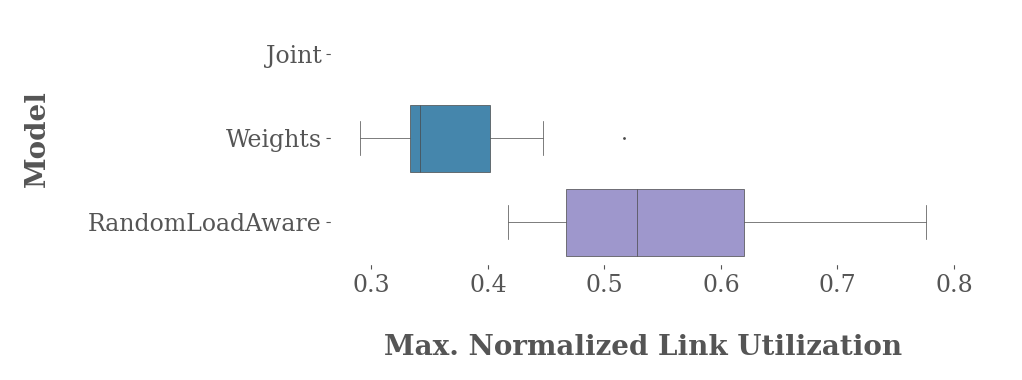
\includegraphics[width=\textwidth]{Report/bilder/RLAPS/results_compare_rla.png}
        \small\textbf{Abb. 5:} Projekt 2 MLU
        \label{fig:enter-label}
\end{center}